\documentclass[border=12pt]{standalone}
\def\pgfsysdriver{pgfsys-dvisvgm.def}
\usepackage[dvisvgm]{xcolor}
\usepackage{xeCJK}
\setCJKmainfont{HaranoAjiGothic-Regular.otf}[BoldFont=HaranoAjiGothic-Bold.otf]
\setCJKsansfont{HaranoAjiGothic-Regular.otf}[BoldFont=HaranoAjiGothic-Bold.otf]
\usepackage{amsmath,amssymb,tikz,lmodern}
\usetikzlibrary{arrows.meta,positioning,calc,fit,backgrounds}
\renewcommand{\familydefault}{\sfdefault}
\definecolor{ink}{HTML}{25322F}
\definecolor{green}{HTML}{246657}
\definecolor{tint}{HTML}{EEF4F0}
\definecolor{soft}{HTML}{C6D2CC}
\definecolor{muted}{HTML}{52615B}
\newif\ifJapanese
\newcommand{\Tx}[2]{\ifJapanese #1\else #2\fi}
\newcommand{\Eff}{\overline{\operatorname{Eff}}}
\newcommand{\heading}[3]{{\color{green}\bfseries #1\quad\Tx{#2}{#3}}\\[5pt]}
% A white rectangle makes the complete citation label clickable, including spaces.
\newcommand{\refurl}[2]{\special{dvisvgm:raw <a xlink:href="#1" target="_blank" rel="noopener noreferrer">}{\setlength{\fboxsep}{0pt}\colorbox{white}{\color{green}\underline{\strut #2}}}\special{dvisvgm:raw </a>}}
\newcommand{\refedge}[3]{\refurl{\csname source#1\endcsname\string##page=#2}{#3}}
\newcommand{\SF}[2]{\refedge{sf}{#1}{#2}}
% GitHub's file preview does not support PDF page fragments.
\newcommand{\LA}[2]{\refurl{\sourcela}{#2}}
\newcommand{\Sch}[2]{\refedge{sch}{#1}{#2}}
\newcommand{\PS}[2]{\refedge{ps}{#1}{#2}}
\tikzset{
 card/.style={draw=soft,fill=white,rounded corners=2pt,align=left,text=ink,font=\fontsize{10.5}{14}\selectfont,inner xsep=12pt,inner ysep=10pt,text width=14.4cm},
 half/.style={card,text width=6.45cm,minimum height=2.05cm},
 result/.style={card,draw=green,fill=tint,line width=.9pt},
 reason/.style={align=left,text=muted,font=\fontsize{9}{12}\selectfont,inner sep=0pt,text width=12.7cm},
 branchreason/.style={reason,text width=5.95cm},
 edge/.style={-{Stealth[length=2.4mm]},draw=green,line width=1pt},
 wire/.style={draw=green,line width=1pt},
}
% Keep the arrow in a dedicated left gutter; explanations never cover it.
\newcommand{\flow}[3]{
 \coordinate (#2-from) at ($(#1.south)+(-6.9,0)$);
 \coordinate (#2-to) at ($(#2.north)+(-6.9,0)$);
 \draw[edge] (#2-from)--(#2-to);
 \node[reason,anchor=west] (#2-reason) at ($(#2-from)!.5!(#2-to)+(.55,0)$) {#3};
}
\newcommand{\Cite}[2]{\refurl{\csname source#1\endcsname}{#2}}

\Japanesetrue
\newcommand{\sourcemm}{https://github.com/openai/math/blob/adc7f1241b42e322a6451854ab7e4b4c146bf78a/preprints/Minimal-metrics-and-interior-injectivity-for-nef-adjoints-September-27-2026/paper.pdf}
\newcommand{\sourcefuj}{https://ems.press/content/serial-article-files/41145}
\newcommand{\sourcedem}{https://www-fourier.univ-grenoble-alpes.fr/~demailly/manuscripts/analmeth_book.pdf}
\newcommand{\sourcelp}{https://arxiv.org/pdf/1809.02500v4}
\newcommand{\sourcegm}{https://www.numdam.org/item/10.24033/asens.2325.pdf}
\begin{document}
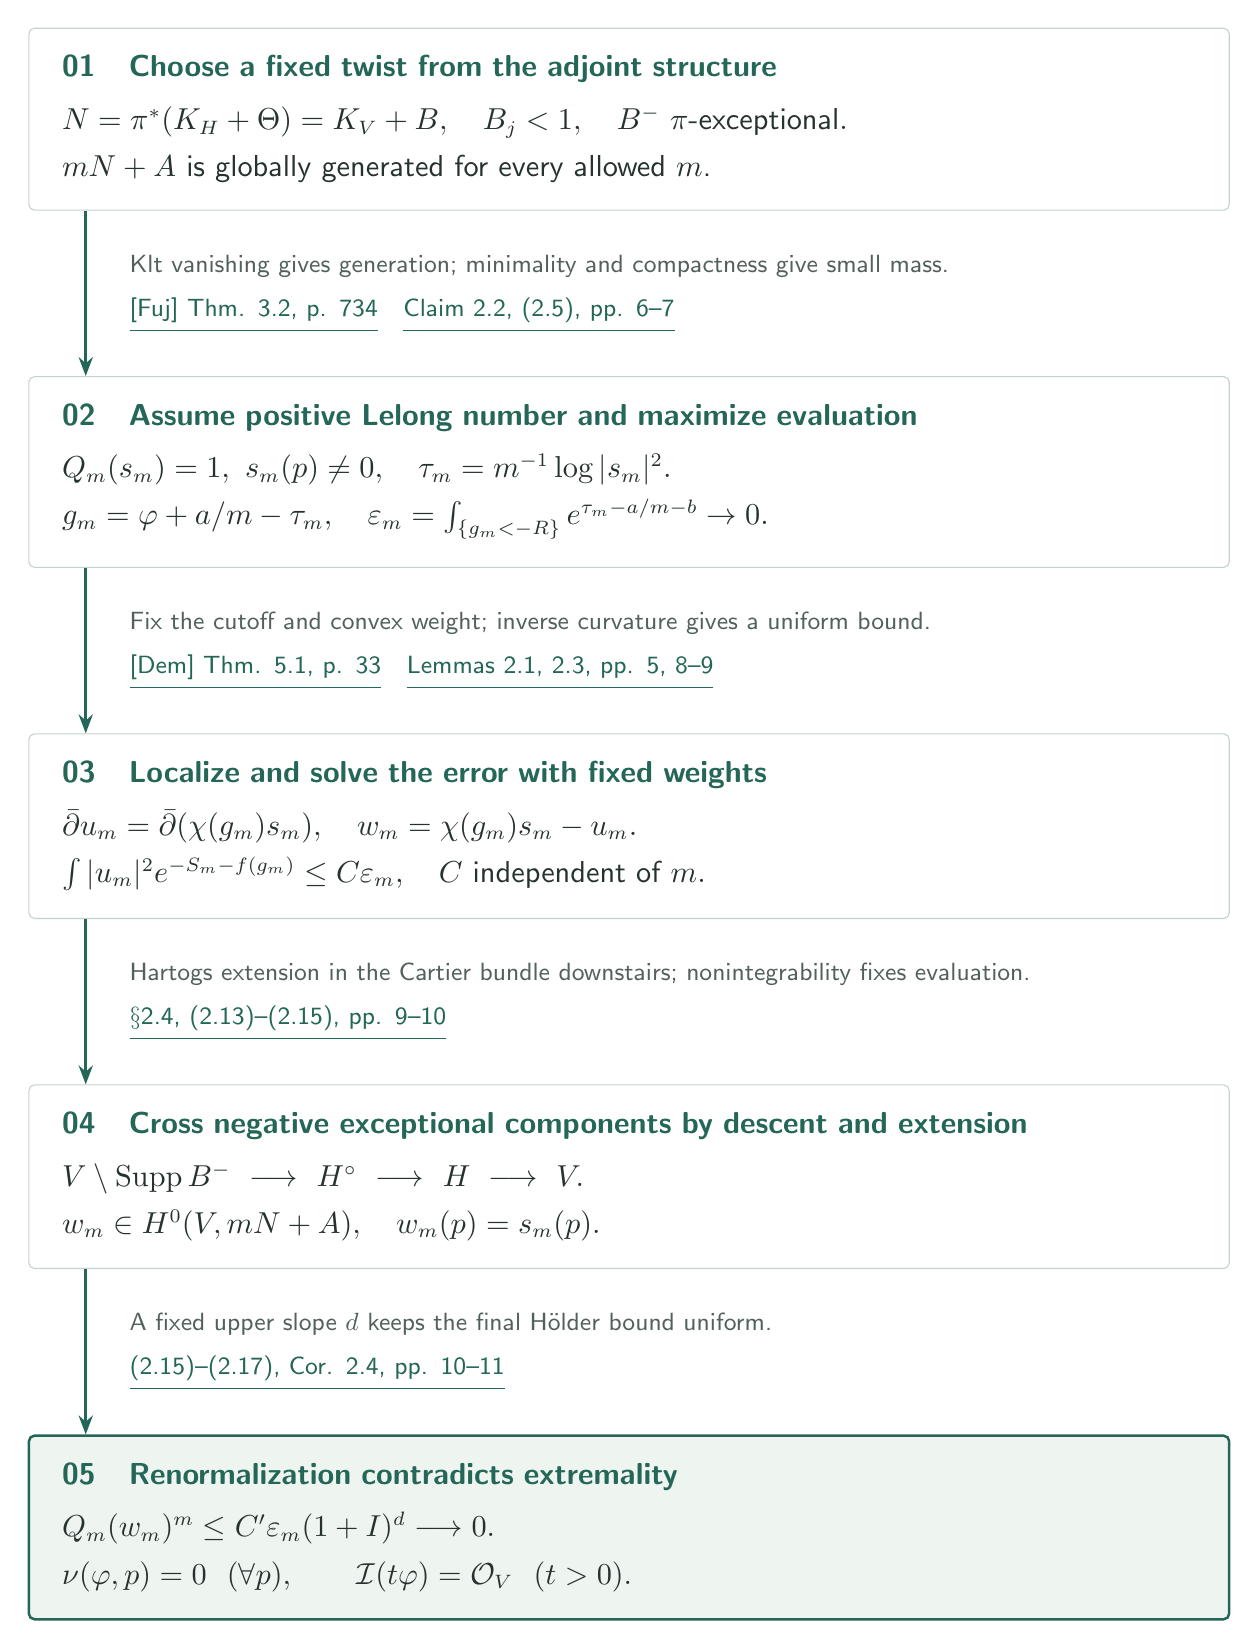
\begin{tikzpicture}
\node[card] (n0) {\heading{01}{随伴構造から固定捻りを選ぶ}{Choose a fixed twist from the adjoint structure}\Tx{$N=\pi^*(K_H+\Theta)=K_V+B,\quad B_j<1,\quad B^-\ \pi\text{-exceptional}.$\\[3pt]$mN+A$ は許されたすべての $m$ で大域生成。}{$N=\pi^*(K_H+\Theta)=K_V+B,\quad B_j<1,\quad B^-\ \pi\text{-exceptional}.$\\[3pt]$mN+A$ is globally generated for every allowed $m$.}};
\node[card,below=2.1cm of n0] (n1) {\heading{02}{正のLelong数を仮定し極値切断を取る}{Assume positive Lelong number and maximize evaluation}\Tx{$Q_m(s_m)=1,\ s_m(p)\ne0,\quad \tau_m=m^{-1}\log|s_m|^2.$\\[3pt]$g_m=\varphi+a/m-\tau_m,\quad\varepsilon_m=\int_{\{g_m<-R\}}e^{\tau_m-a/m-b}\to0.$}{$Q_m(s_m)=1,\ s_m(p)\ne0,\quad \tau_m=m^{-1}\log|s_m|^2.$\\[3pt]$g_m=\varphi+a/m-\tau_m,\quad\varepsilon_m=\int_{\{g_m<-R\}}e^{\tau_m-a/m-b}\to0.$}};
\flow{n0}{n1}{\Tx{klt消滅で大域生成。極小性と正規化された重みのコンパクト性を使う。}{Klt vanishing gives generation; minimality and compactness give small mass.}\\[4pt]\Cite{fuj}{[Fuj] Thm. 3.2, p. 734}\quad \Cite{mm}{Claim 2.2, (2.5), pp. 6--7}}
\node[card,below=2.1cm of n1] (n2) {\heading{03}{固定重みで局所化し誤差を解く}{Localize and solve the error with fixed weights}\Tx{$\bar\partial u_m=\bar\partial(\chi(g_m)s_m),\quad w_m=\chi(g_m)s_m-u_m.$\\[3pt]$\int|u_m|^2e^{-S_m-f(g_m)}\le C\varepsilon_m,\quad C\text{ は }m\text{ に依存しない。}$}{$\bar\partial u_m=\bar\partial(\chi(g_m)s_m),\quad w_m=\chi(g_m)s_m-u_m.$\\[3pt]$\int|u_m|^2e^{-S_m-f(g_m)}\le C\varepsilon_m,\quad C\text{ independent of }m.$}};
\flow{n1}{n2}{\Tx{固定したカットオフと凸重み。逆曲率積分で定数を一様にする。}{Fix the cutoff and convex weight; inverse curvature gives a uniform bound.}\\[4pt]\Cite{dem}{[Dem] Thm. 5.1, p. 33}\quad \Cite{mm}{Lemmas 2.1, 2.3, pp. 5, 8--9}}
\node[card,below=2.1cm of n2] (n3) {\heading{04}{負の例外成分を降下と延長で越える}{Cross negative exceptional components by descent and extension}\Tx{$V\setminus\operatorname{Supp}B^-\ \longrightarrow\ H^\circ\ \longrightarrow\ H\ \longrightarrow\ V.$\\[3pt]$w_m\in H^0(V,mN+A),\quad w_m(p)=s_m(p).$}{$V\setminus\operatorname{Supp}B^-\ \longrightarrow\ H^\circ\ \longrightarrow\ H\ \longrightarrow\ V.$\\[3pt]$w_m\in H^0(V,mN+A),\quad w_m(p)=s_m(p).$}};
\flow{n2}{n3}{\Tx{基底のCartier束でHartogs延長。非可積分性が点での値を固定する。}{Hartogs extension in the Cartier bundle downstairs; nonintegrability fixes evaluation.}\\[4pt]\Cite{mm}{$\S$2.4, (2.13)--(2.15), pp. 9--10}}
\node[result,below=2.1cm of n3] (n4) {\heading{05}{正規化し直すと極値性に矛盾する}{Renormalization contradicts extremality}\Tx{$Q_m(w_m)^m\le C^\prime\varepsilon_m(1+I)^d\longrightarrow0.$\\[3pt]$\nu(\varphi,p)=0\ \ (\forall p),\qquad\mathcal I(t\varphi)=\mathcal O_V\ \ (t>0).$}{$Q_m(w_m)^m\le C^\prime\varepsilon_m(1+I)^d\longrightarrow0.$\\[3pt]$\nu(\varphi,p)=0\ \ (\forall p),\qquad\mathcal I(t\varphi)=\mathcal O_V\ \ (t>0).$}};
\flow{n3}{n4}{\Tx{固定した上側勾配 $d$ によりHölder評価の定数を一様化する。}{A fixed upper slope $d$ keeps the final Hölder bound uniform.}\\[4pt]\Cite{mm}{(2.15)--(2.17), Cor. 2.4, pp. 10--11}}
\end{tikzpicture}
\end{document}
